\documentclass[tikz]{standalone}
\usetikzlibrary{calc,patterns,angles,quotes,intersections,positioning,decorations.markings}
\usepackage{pgfplots}
\pgfplotsset{compat=newest}

\pagestyle{empty}

\begin{document}
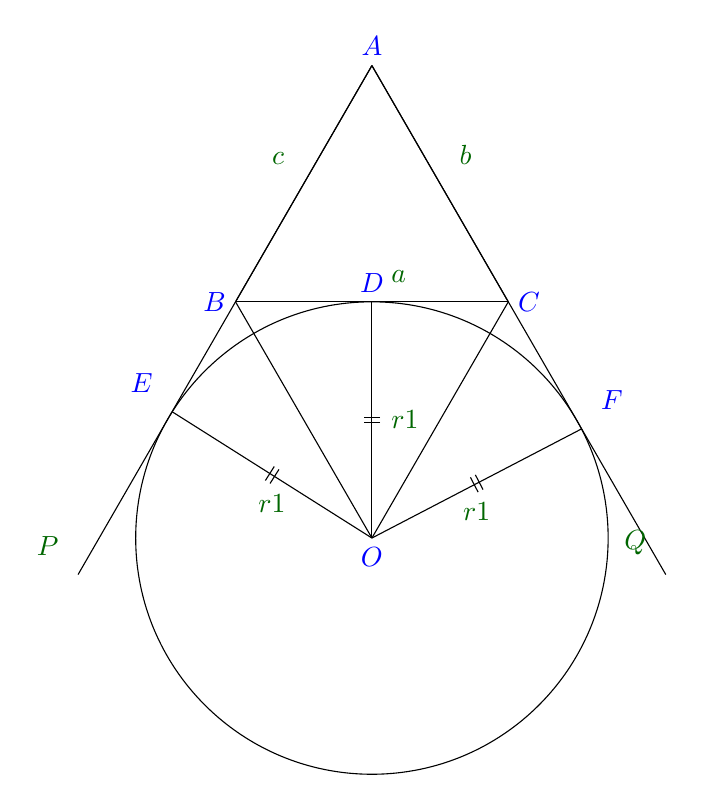
\begin{tikzpicture}[
decoration={
  markings,
  mark=at position 0.5 with
  {
    \draw (-1pt,-3pt) -- ++(0,6pt);
    \draw (1pt,-3pt) -- ++(0,6pt);
  }
}
]
  \draw[name path=Circle] (0, -4) circle [radius=3];
  \coordinate [label={[blue]above:$A$}] (A) at (0, 2);
  \coordinate [label={[blue]right:$C$}] (C) at (1.732, -1);
  \coordinate [label={[blue]left:$B$}] (B) at (-1.732, -1);
  \coordinate [label={[blue]below:$O$}] (O) at (0, -4);
  \coordinate [label={[blue]above:$D$}] (D) at (0, -1);
  \draw (B) -- (C);
  \draw (A) -- (B);
  \draw (C) -- (A);
  \draw[postaction=decorate] (O) -- (D);
  \draw (O) -- (B);
  \draw (O) -- (C);
  \draw [name path=AB] (A) -- ($(B)!-4cm!(A)$);
  \draw [name path=AC] (A) -- ($(C)!-4cm!(A)$);
  \path[name intersections={of=AB and Circle,by={E}}]
  node[label={[blue]above left:$E$}] at (E) {};
  \path[name intersections={of=AC and Circle,by={F}}]
  node[label={[blue] above right:$F$}] at (F) {};
  \draw[postaction=decorate] (O) -- (E);
  \draw[postaction=decorate] (O) -- (F);
  \node[label={[black!60!green] above right:$a$}] at ( $ (B)!0.5!(C) $ ) (l1) {};
  \node[label={[black!60!green] above right:$b$}] at ( $ (A)!0.5!(C) $ ) (l2) {};
  \node[label={[black!60!green] above left:$c$}] at ( $ (A)!0.5!(B) $ ) (l3) {};
  \node[label={[black!60!green] above left:$P$}] at ( $(B)!-4cm!(A)$ ) (l4) {};
  \node[label={[black!60!green] above left:$Q$}] at ( $(C)!-4cm!(A)$ ) (l5) {};
  \node[label={[black!60!green] right:$r1$}] at ( $ (O)!0.5!(D) $ ) (l1) {};
  \node[label={[black!60!green] below:$r1$}] at ( $ (O)!0.5!(E) $ ) (l1) {};
  \node[label={[black!60!green] below:$r1$}] at ( $ (O)!0.5!(F) $ ) (l1) {};
\end{tikzpicture}
\end{document}
